\chapter{Related Work}
This chapter will give an overview into the background and concepts of this thesis.
In the first section the Internet of Things an related subtopics like Smart Factories and Smart Cities are considered.
Cyber Physical Systems, which are important for the development of Smart Factories are also covered in this section.
Virtualization in general is the main topic of the second section.
First we dive into the area of Virtual Machines, followed by Container Virtualization.
Both are related to each other and sharing some basic ideas.
Container Orchestration as an own subsection show some possibilites of Container Virtualization.
The last subsection Network Function Virtualization concludes with an introduction into the virtualization of network node functions to create communication services.


\section{Internet of Things}
The \ac{IoT} has been a subject of great media- and economically growth in the recent years.
In the year 2008 the number of devices which are connected to the internet was higher than the human population.\cite{Eva11}
Cisco Internet Business Solutions Group predicted that the number will grow up to 50 billion in 2020, this equates to around 6 devices per person.\cite{Eva11}
Most of today\'s interactions are \ac{H2H} or \ac{H2M} communication.
The \ac{IoT} on the other hand aim for the \ac{M2M} communication.
This allows every physical devices to be interconnected and to communicate with each other.
These devices are also called "Smart Devices".
Craeting a network where all physical objects and people are connected via software is one primary goal of the \ac{IoT}.\cite{Rui2015}\cite{Kra13}
When objects are able to capture and monitor their environment, a network can perceive external stimuli and respond to them.\cite[p. 40]{Itu11}
Therefore a new dimension of information and communication technology will be created, where users have access to everything at any time, everywhere.
In addition to smart devices, subcategories are also emerging from the internet of things which, in addition to the physical devices, also describe technologies such as protocols and infrastructures.
The "`Smart Home"' has been a prominent topic in media and business for many years.
SmartCity or Industrie 4.0 are also becoming established and are increasingly popular.
But the Internet started with the appearance of bar codes and \ac{RFID} chips.\cite{Kra13}
The second step, which is more or less the current situation, sensors, physical devices, technical devices, data and software are connected to each other.\cite{Kra13}
This was achieved, in particular, by cloud computing, which provides the highly efficient memory and computing power that is indispensable for such networks.\cite{Rui2015}
The next step could be a "`Cognitive Internet of Things"', which enables easier object and data reuse across application areas, for example through interoperable solutins, high-speed internt connections and a semantic information distribution.\cite{Kra13}
Just as the omnipresent information processing in everday life, also known as "`Ubiquitous Computing"', which was first mentioned in the "`The Computer for the 21st Century"'\cite{Wei91} by Marks Weiser, it will take some time until it is ubiquitous.


\subsection{Industry 4.0 and Smart Factories}

The industry as an changing environment is currently in the state of the so called "fourth industrial revolution".
The first industrial revolution was driven by steam powered machines.
Mass production and division of labor was the primary improvement of the second industrial revolution, whereas the third revolution was characterized by using electronics and the integration of \ac{IT} into manufacturing processes.\cite[p. 1]{Lom2016}
In the recent years the size, cost and power consumption of chipsets are reduced which made it possible to embed sensors into devices and machines much easier and cheaper.\cite[p. 1]{Brito2016}
The "Industrie 4.0" is the fourth step in this evolution and was first mentioned at the Hannover Fair in 2011.\cite[p. 1]{Lom2016}
"Industrie 4.0 is a collective term for technologies and concepts of value chain organization."\cite[p. 11]{Her2015}
Main components of a Smart Factory are \ac{CPS}, \ac{IoT}, \ac{IoS}, \ac{IoP} and \ac{IoE}.\cite[p. 11]{Her2015}

\begin{table}[htpb]
  \centering
  \begin{tabular}{| r | c c c c |}
  	\rowcolor{dunkelgrau}
  	\hline
  	                      & Cyber-Physical & Internet  & Internet    & Smart Factory \\
    \rowcolor{dunkelgrau}
                          & Systems        & of Things & of Services &  \\
  	\hline
  	Interoperability      & X        & X        & X          & X    \\
  	Virtualization        & X        & -        & -          & X    \\
    Decentralization      & X        & -        & -          & X    \\
    Real-Time Capability  & -        & -        & -          & X    \\
    Service Orientation   & -        & -        & X          & -    \\
    Modularity            & -        & -        & X          & -    \\
  	\hline
  \end{tabular}
  \caption[Design principles of each Industry 4.0 component]{Design principles of each Industry 4.0 component.\cite[p. 11]{Her2015}}
  \label{tab:industryComponents}
\end{table}

Table \ref{tab:industryComponents} shows the six design principles which can be from the Industrie 4.0 components.
They can help companies to identify and implement Industry 4.0 scenarios.\cite[p. 11]{Her2015}

\begin{enumerate}
  \item \textit{Interoperability} \ac{CPS} of various manufacturers are connected with each other. Standards will be the key success factor in this area.\cite[p. 11]{Her2015}
  \item \textit{Virtualization} \ac{CPS} are able to monitor physical processes via sensors. The resulting data is linked to virtual plant and simulation models. These models are virtual copyies of physical world entities.\cite[p. 11]{Her2015}
  \item \textit{Decentralization} \ac{CPS} are able to make decisions on their own, for example when \ac{RFID} chips send the necessary working steps to the machine. Only in cases of failure the systems delegate task to a higher level.\cite[p. 11]{Her2015}
  \item \textit{Real-Time Capability} Data has to be collected and analyzed in real time and the status of the plant is permanently tracked and analyzed. This enables the \ac{CPS} to react to a failure of a machine and can reroute the products to another machine.\cite[p. 11]{Her2015}
  \item \textit{Service Orientation} \ac{CPS} are available over the \ac{IoS} and can be offered both internally and across company borders to different participants. The manufacturing process can be composed based on specific customer requirements.\cite[p. 11]{Her2015}
  \item \textit{Modularity} The system is able to be adjusted in case of seasonal fluctuations or changed product characteristics, by replacing or expanding individual modules.\cite[p. 11]{Her2015}
\end{enumerate}

% Gute Quelle:
% http://winfwiki.wi-fom.de/index.php/Wertsch%C3%B6pfungsnetzwerke_und_Industrie_4.0

Another important aspect of Industry 4.0 is implementation of the digital structure of Smart Factory.
The vertical integration contains the connection and communication of subsystems within the factory enables flexible and adaptable manufacturing systems.\cite[p. 7 ff.]{Vbw2014}
The horizontal integration enables technical processes to be integrated in cross-company business processes and to be synchronized in real time through multiple participants.\cite[p. 7 ff.]{Vbw2014}

\todo{mehr schreiben}
\todo{Infographik ?}


\subsection{Cyber Physical Systems}

\todo{"These advancements
benefit the development of Cyber-Physical Systems (CPSs),
a technology where every physical entity has a digital twin
or avatar in the virtual world, also facilitate the move from
centralized control, configuration and management of machines
to autonomous and decentralized solutions." \cite{brito1}

"Cyber-Physical Systems (CPSs), a technology where every
physical entity has a digital twin or avatar in the virtual
world. It also facilitates the move from centralized control,
configuration and management of machines to autonomous
and decentralized solutions. The application of CPS’s
concepts in the Shop Floor brings an essential framework
to the development of Smart Factories, but the technology
still needs improvements and maturity." \cite{brito2}

"CPS comes as a concept that foreseen the
digitization of physical systems allowing its representation
in the virtual world [19], and this is becoming possible due
to achievements made in different fields, such as embedded
systems, miniaturization, and network technologies, to cite
some." \cite{brito2}

"The important part of the Industry 4.0 is the Cyber-Physical
System (CPS), networking machines and components with the
additional intelligent and highly flexible software. CPSs are
connected with embedded systems, these being parts of complete
devices with real-time computing constraints. CPSs link such
embedded systems to digital networks facilitating independent
data processing. The assignment of an IP address allows such
systems to be controlled and monitored online (the Figure 4 shows
the basic principles of CPS). Owing to such embedded computer
systems, sensors and actuators, cyber-physical systems organize
production automatically and autonomously [18]. Central process
control can be eliminated as it can be taken over by CPS-based
components. This concept of a value chain organization is also
referred not to the Industry 4.0, but also smart city, where each
component should behave in the same way. CPS can be
considered as the first common area that connects the smart city
and Industry 4.0 factory to the whole forming a mutual symbiosis."\cite{Lom}}


\subsection{Fog Computing}


\section{Virtualization}


\subsection{Virtual Machines}


\subsection{Container Virtualization}


\subsubsection{Docker}

\todo{"First, we must know what exactly Docker is and does. Docker is a container managment system that helps easily manage Linux Container (LXC) in an easier and unversal fashion. This lets you create images in virtual environment ons your laptop and run commands or operations against them. The actions you do to the containers that you run in these environments locally on your own machine will be the same commands or operations you run against them when they are running in your production environment. This helps in not having to do things differently when you go from a development environment like that on your local machine to  a production environemnt like that on your local machine to a production environemnt on your server. Now, let's take a look at the differences between Docker containers and the typical virtual machine environments.

In the followin illustration, we can see the typical Docker setup on the right-hand side versus the typical VM setup on the left-hand side:}
\begin{figure}
    \centering
    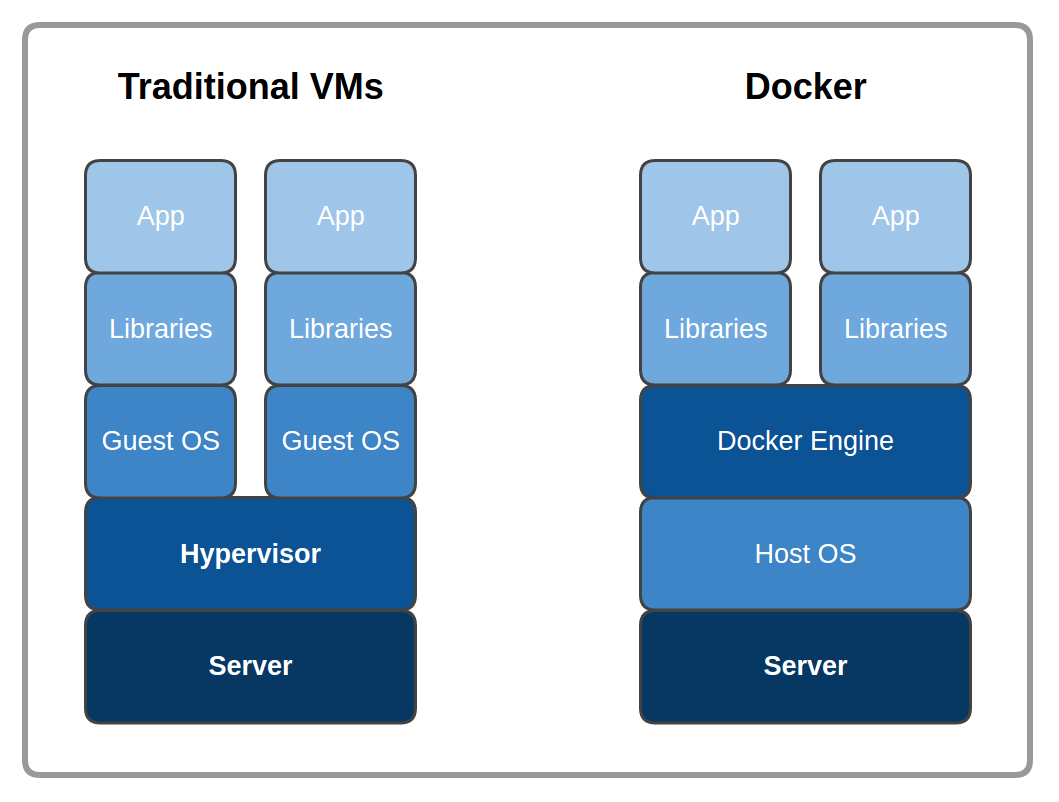
\includegraphics[width=0.6\textwidth]{resources/images//docker_vs_vm.png}
    \caption[Structure traditional VMs vs. Docker]{Structure traditional VMs vs. Docker. Adapted from: \cite{Gal2015}, p. 2}
    \label{fig:vms_vs_docker}
\end{figure}

\todo{"This illustration gives us a lot of insight into the biggest key benefit of Docker, that is, there is no nedd for a complete operating system every titme we need to bring up a new container, which cuts down on the overall size of containers. Docker relies on using the host OS's Linux kernel (since almost all the versions of Linux use the standard kernel models) fot he OS it was build upon, such as Red Hat, CentOS, Ubuntu, and so on. For this reason, you can have almost any Linux OS as your host operationg system (Ubuntu in the previous illustartion) and be able to layer other OSes on top of the host. For example, in the earlier illustration, we could have Red Hat running for one app (the one on the left) and Debian running for the other app (the on on the right), but there would never be need to actually install Red Hat or Debian on the host. Thus, another benefit of Docker ist the size of aimages when they are born. They are not build with the largest piece: the kernel or the operating sytem. This makes them incredibley small, compact, and easy to ship."\cite{Gal2015}}


\subsection{Container Orchestration}

\subsubsection{Kubernetes}

\subsubsection{Docker Swarm}


\subsection{Network Function Virtualization}


\section{Conclusion}
